\documentclass[a4paper,12pt]{article} 

%Добавляет возможность искать и копировать текст
\usepackage{cmap}

%Убирает пробел между названием таблицы/рисунка и самой таблицей/рисунком
\usepackage{caption}
\captionsetup[table]{skip= -0.5 cm}
\captionsetup[figure]{skip= -0.5 cm}

%Выравнивание названия таблиц по левому краю
%\usepackage[nooneline]{caption} 
%Размеры отступов 
\usepackage[left=20mm, top=20mm, right=20mm, bottom=20mm, footskip=10mm]{geometry}

%Рисунки
\usepackage{graphicx}
\usepackage{wrapfig} %обтекание элементов

%Русский язык в формулах
\usepackage{mathtext}

%  Русский язык
\usepackage[T2A]{fontenc}			
\usepackage[utf8]{inputenc}			
\usepackage[english,russian]{babel}	

%Готические буквы
\usepackage{amssymb}

% Математика
\usepackage{amsmath,amsfonts,amssymb,amsthm,mathtools} 
\usepackage{wasysym}

%Цветные подписи в таблице
\usepackage[table,xcdraw]{xcolor}

\usepackage{fancyhdr} % Колонтитулы
 	\pagestyle{fancy}
 	\renewcommand{\headrulewidth}{0.3mm}  % Толщина линейки, отчеркивающей верхний колонтитул
 	%\lfoot{Нижний левый}
 	%\rfoot{Нижний правый}
 	\rhead{Белостоцкий Артмемий, Б04-006}
 	%\chead{Верхний в центре}
 	\lhead{Лабораторная работа №3.3.4}
 	% \cfoot{Нижний в центре} % По умолчанию здесь номер страницы








\begin{document} 

%Титульник 
\begin{titlepage}
	\begin{center}
		\large 	МИНИСТЕРСТВО ОБРАЗОВАНИЯ И НАУКИ РОССИЙСКОЙ ФЕДЕРАЦИИ\\
				МОСКОВСКИЙ ФИЗИКО-ТЕХНИЧЕСКИЙ ИНСТИТУТ \\
				(НАЦИОНАЛЬНЫЙ ИССЛЕДОВАТЕЛЬСКИЙ ИНСТИТУТ)\\ 
				ФИЗТЕХ-ШКОЛА ЭЛЕКТРОНИКИ, ФОТОНИКИ \\
				И МОЛЕКУЛЯРНОЙ ФИЗИКИ \\
		
		
		\vspace{4.0 cm}
		Лабораторная работа № 3.3.4 \\ 
		\LARGE \textbf{Эффект Холла в полупроводниках}
	\end{center}
	\vspace{3 cm} \large
	
	\begin{flushright}
		выполнил студент 2 курса \\
		{группы Б04-006}\\
		\textbf{Белостоцкий Артемий}\\
	\end{flushright}
	
	\vfill

	\begin{center}
	Долгопрудный, 2021 г.
	\end{center}
\end{titlepage}                                                                      
 
\section{Цель работы}
Исследовать зависимость ЭДС Холла от величины магнитного поля при различных токах через образец для определения константы Холла; определить знак носителей заряда и проводимость материала образца.

\section{В работе используются}
	\begin{itemize}
	\item электромагнит с источником питания GPR;
	\item цифровой вольтметр В7-65/5;
	\item батарейка 1,5 В;
	\item реостат;
	\item миллиамперметр;
	\item образцы легированного германия;
	\item измеритель магнитной индукции ATE-8702;
	\end{itemize}


\section{Экспериментальная установка}
	\begin{figure}[h]
		\begin{center}
		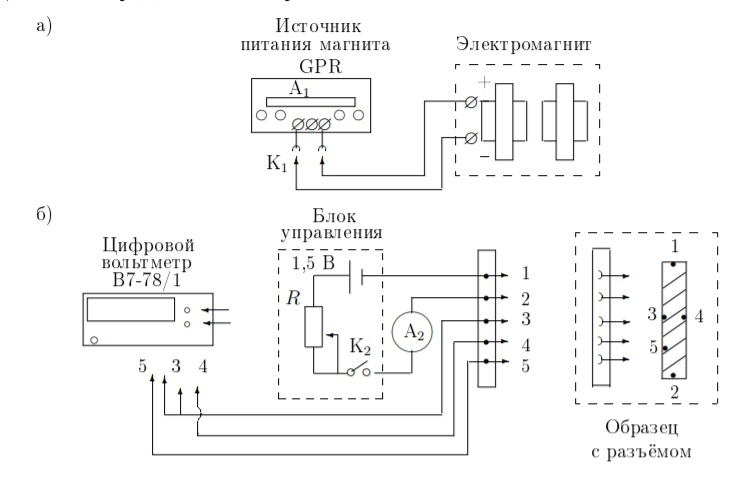
\includegraphics[scale=0.5]{fig1}
		\end{center}
		\caption{Схема установки для исследования эффекта Холла в полупроводниках}
		\end{figure}

Схема для измерения ЭДС Холла представлена на рисунке. В зазоре электромагнита создаётся постоянное магнитное поле, величину которого можно менять регуляторами источника питания электромагнита. Градуировка магнита проводится при помощи милливеберметра.\\

\newpage	

Образец из легированного германия, смонтированный в специальном держателе, подключается к источнику питания. При замыкании К$_2$ вдоль длинной стороны образца течёт ток, величина которого регулируется реостатом $R$ и измеряется миллиамперметром. В образце, помещённом в зазор, возникает разность потенциалов $U_{34}$, которая измеряется с помощью цифрового вольтметра.

 Влияние омического падения напряжения исключается измерением напряжения $U_0$ между 3 и 4 в отсутствие магнитного поля. По знаку $\mathcal{E} = U_{34} \pm U_0$ можно определить характер проводимости -- электронный или дырочный, зная напрявление тока в образце и напрвление магнитного поля.
 
 Померив ток $I_{35}$ в образце и напряжение $U_{35}$ между контактами 3 и 5 в отсутствие магнитного поля можно рассчитать проводимость материала по формуле
\begin{equation}
\lambda = \frac{IL_{35}}{U_{35}al},
\end{equation}
где $L_{35}$ -- расстояние между контактами 3 и 5, а $a$ и $l$ -- толщина и ширина образца.

\section{Ход работы}
\subsection*{Градуировка электромагнита}

Изменяя ток в обмотке электромагнита $ I_M $, с помощь. измерителя магнитной индукции исследуем зависимость $B(I_M)$ данные занесем в Таблицу 1:

\begin{table}[h]
\caption{}
\begin{center}
\begin{tabular}{|
>{\columncolor[HTML]{92D050}}c |c|c|c|c|c|c|c|c|}
\hline
\textbf{I, мА}  & 0 & 0,2   & 0,4   & 0,6 & 0,8   & 1   & 1,2    & 1,4  \\ \hline
\textbf{B, мТл} & 0 & 206,7 & 433,6 & 642 & 814,3 & 913 & 1018,8 & 1076 \\ \hline
\end{tabular}
\end{center}
\end{table}
По данным Таблицы 1 построим график зависимости $B(I_M)$
	\begin{figure}[h]
		\begin{center}
		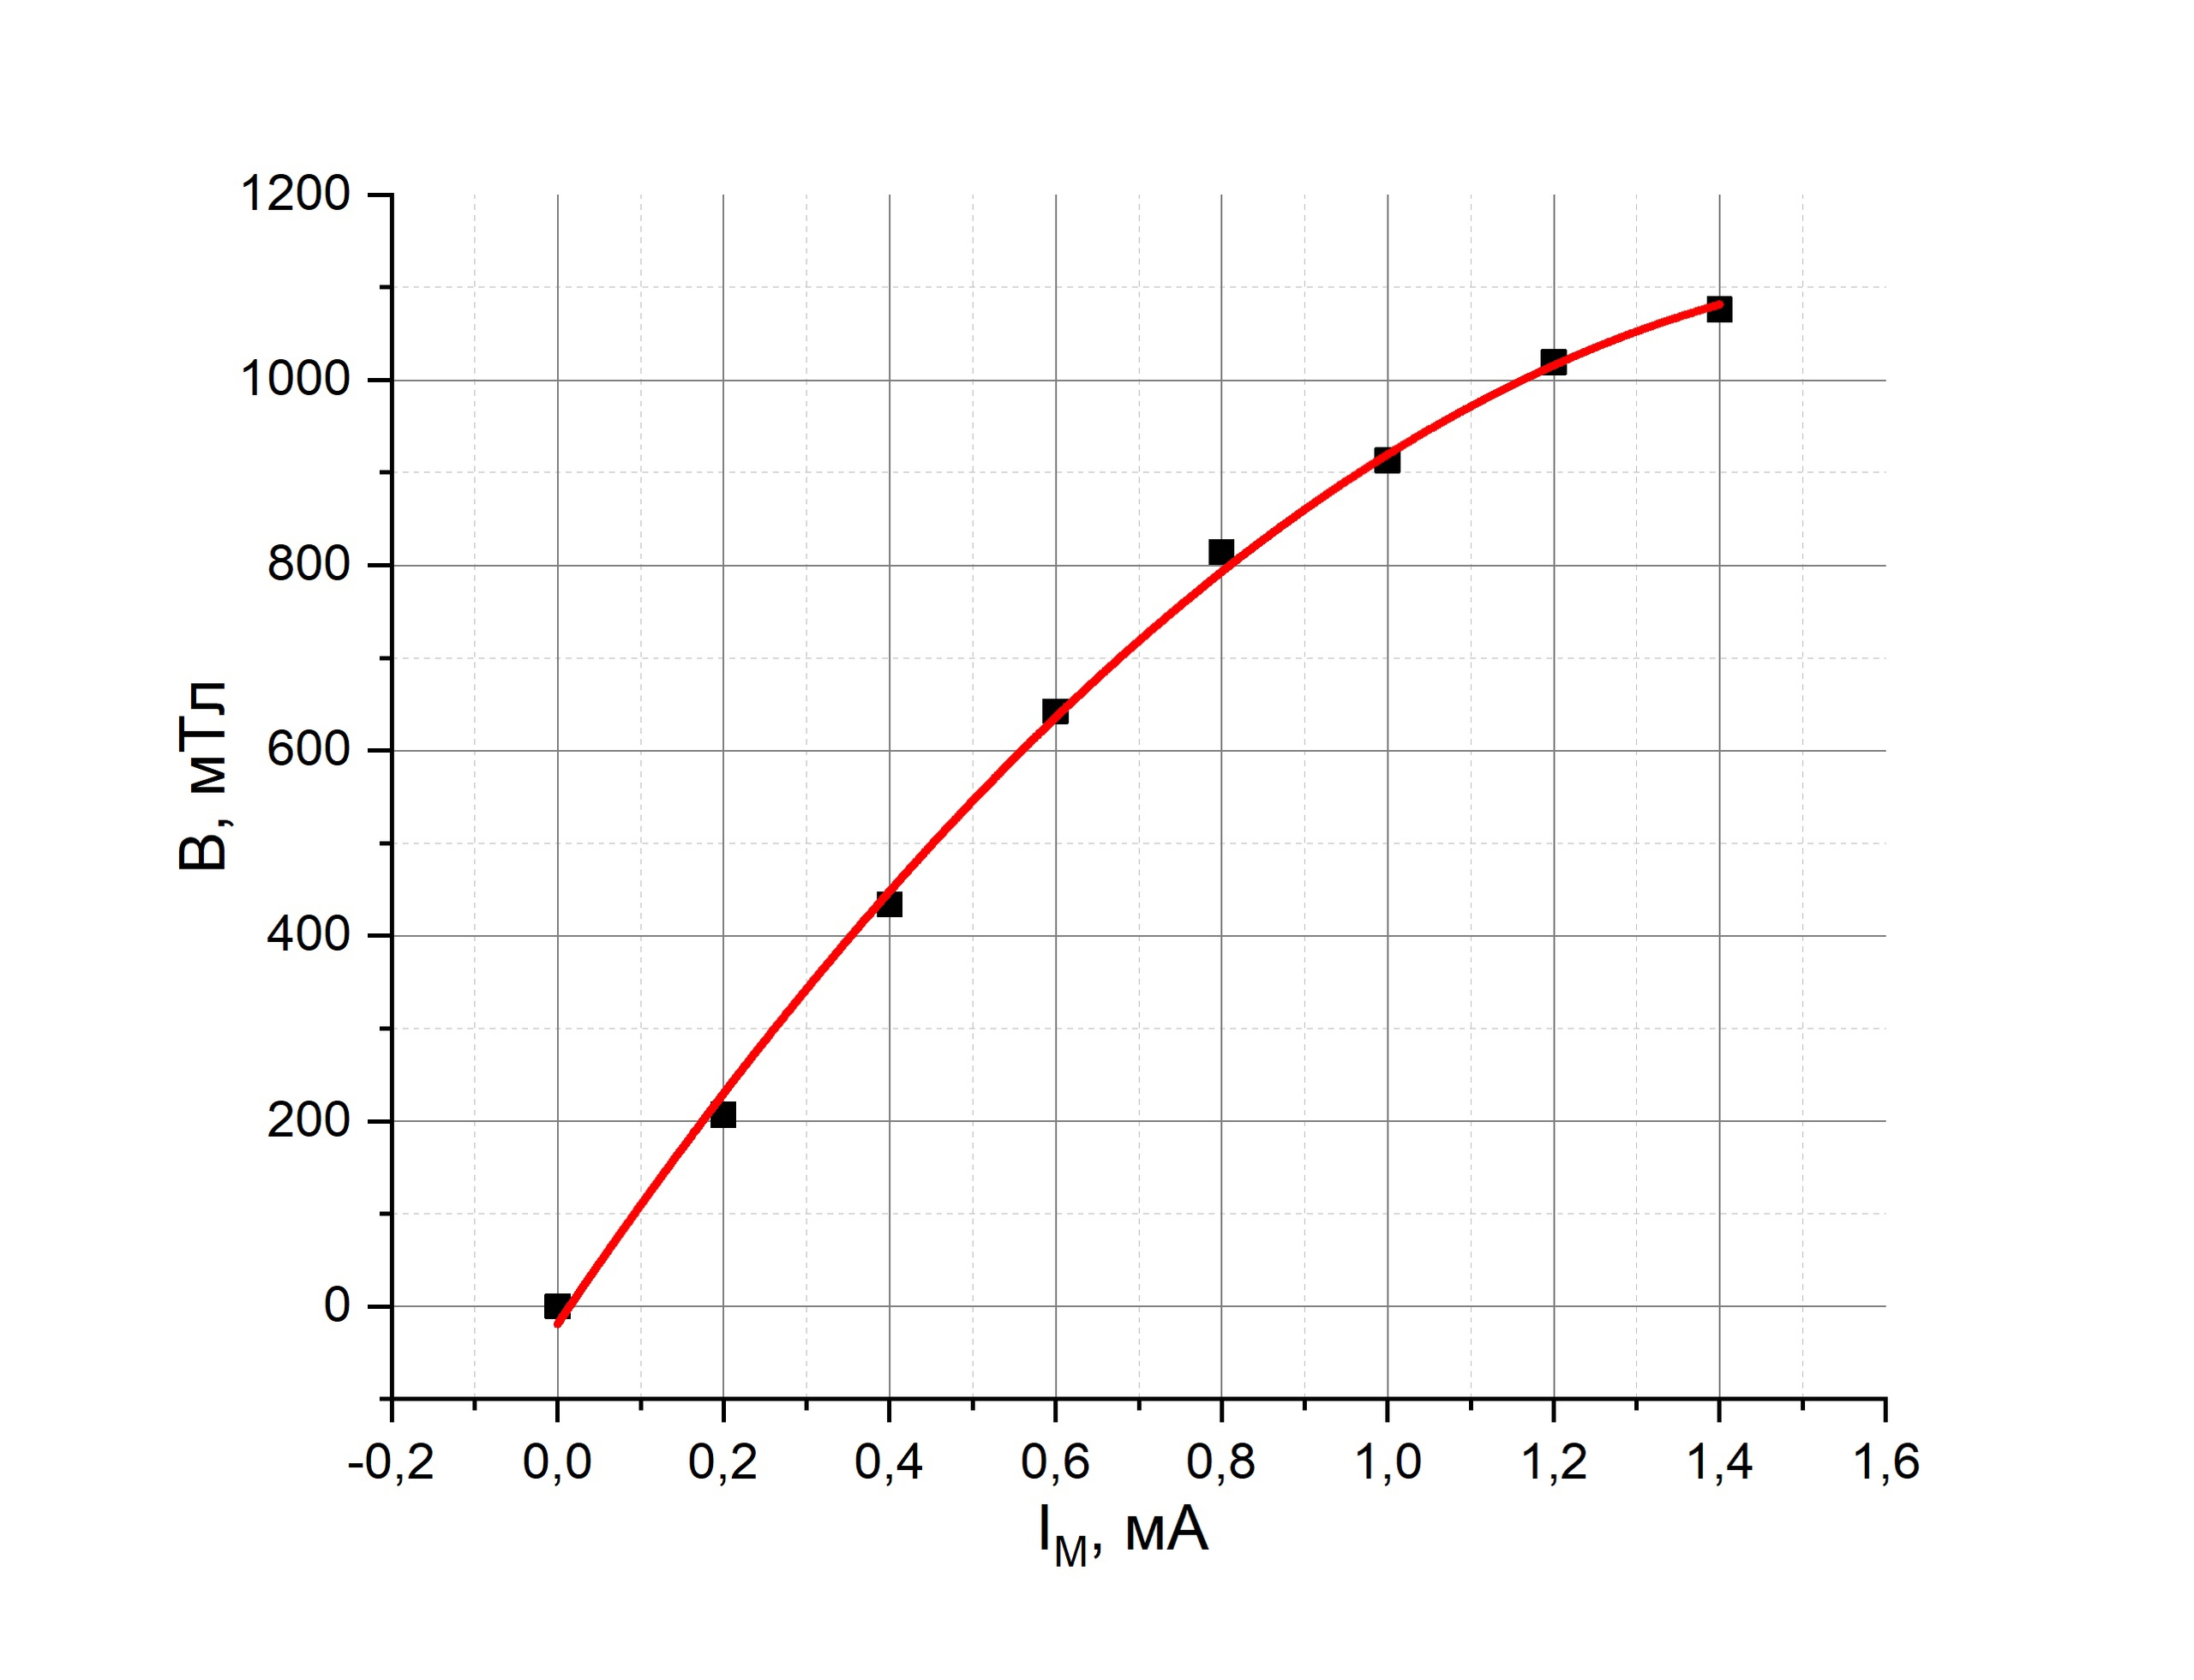
\includegraphics[scale=0.11]{graph1}
		\end{center}
		\caption{Зависимость $B(I_M)$}
		\end{figure}

\subsection*{Измерение ЭДС Холла}

Вставим держатель с образцом в зазор электромагнита и установим минимальное значение тока через образец $I \approx 0,3 мА$.В отсутствие магнитного поля вольтметр показывает небольшое напряжение $U_0$, вызванное несовершенством контактов 3,4 и проводками.

Снимем зависимость напряжения U от тока $I_M$ при разных токах через образец -- I.ЭДС Холла будет определятся формулой $\varepsilon = U - U_0 $.` Данные занесем в таблицы
\begin{table}[h!]
\caption{I = 0,3 мА}
\begin{center}
\begin{tabular}{|
>{\columncolor[HTML]{92D050}}l |l|l|l|l|l|l|l|}
\hline
\textbf{$\varepsilon$, мкВ} & 10  & 22  & 33  & 43  & 50 & 55  & 58  \\ \hline
\textbf{$I_M$, мА} & 0,2 & 0,4 & 0,6 & 0,8 & 1  & 1,2 & 1,4 \\ \hline
\end{tabular}
\end{center}
\end{table}

\begin{table}[h!]
\caption{I = 0,4 мА}
\begin{center}
\begin{tabular}{|
>{\columncolor[HTML]{92D050}}l |l|l|l|l|l|l|l|}
\hline
\textbf{$\varepsilon$, мкВ} & 15  & 30  & 45  & 58  & 68 & 74  & 79  \\ \hline
\textbf{$I_M$, мА} & 0,2 & 0,4 & 0,6 & 0,8 & 1  & 1,2 & 1,4 \\ \hline
\end{tabular}
\end{center}
\end{table}
\begin{table}[h!]
\caption{I = 0,5 мА}
\begin{center}
\begin{tabular}{|
>{\columncolor[HTML]{92D050}}l |l|l|l|l|l|l|}
\hline
\textbf{$\varepsilon$, мкВ} & 19  & 38  & 57  & 74  & 85 & 95  \\ \hline
\textbf{$I_M$, мА} & 0,2 & 0,4 & 0,6 & 0,8 & 1  & 1,2 \\ \hline
\end{tabular}
\end{center}
\end{table}

\begin{table}[h!]
\caption{I = 0,6 мА}
\begin{center}
\begin{tabular}{|
>{\columncolor[HTML]{92D050}}l |l|l|l|l|l|l|}
\hline
\textbf{$\varepsilon$, мкВ} & 22  & 45  & 69  & 87  & 100 & 110 \\ \hline
\textbf{$I_M$, мА} & 0,2 & 0,4 & 0,6 & 0,8 & 1   & 1,2 \\ \hline
\end{tabular}
\end{center}
\end{table}

\begin{table}[h!]
\caption{I = 0,7 мА}
\begin{center}
\begin{tabular}{|
>{\columncolor[HTML]{92D050}}l |l|l|l|l|l|l|}
\hline
\textbf{$\varepsilon$, мкВ} & 26  & 54  & 79  & 102 & 119 & 129 \\ \hline
\textbf{$I_M$, мА} & 0,2 & 0,4 & 0,6 & 0,8 & 1   & 1,2 \\ \hline
\end{tabular}
\end{center}
\end{table}

\begin{table}[h!]
\caption{I = 0,8 мА}
\begin{center}
\begin{tabular}{|
>{\columncolor[HTML]{92D050}}l |l|l|l|l|l|l|}
\hline
\textbf{$\varepsilon$, мкВ} & 30  & 60  & 91  & 116 & 134 & 148 \\ \hline
\textbf{$I_M$, мА} & 0,2 & 0,4 & 0,6 & 0,8 & 1   & 1,2 \\ \hline
\end{tabular}
\end{center}
\end{table}

\newpage

\begin{table}[h!]
\caption{I = 0,9 мА}
\begin{center}
\begin{tabular}{|
>{\columncolor[HTML]{92D050}}l |l|l|l|l|l|l|}
\hline
\textbf{$\varepsilon$, мкВ} & 32  & 68  & 101 & 130 & 151 & 166 \\ \hline
\textbf{$I_M$, мА} & 0,2 & 0,4 & 0,6 & 0,8 & 1   & 1,2 \\ \hline
\end{tabular}
\end{center}
\end{table}

Построим семейство характеристик $\varepsilon = f(B)$ при разных значениях тока через образец I по данным Таблиц 2 - 8.
	\begin{figure}[h]
		\begin{center}
		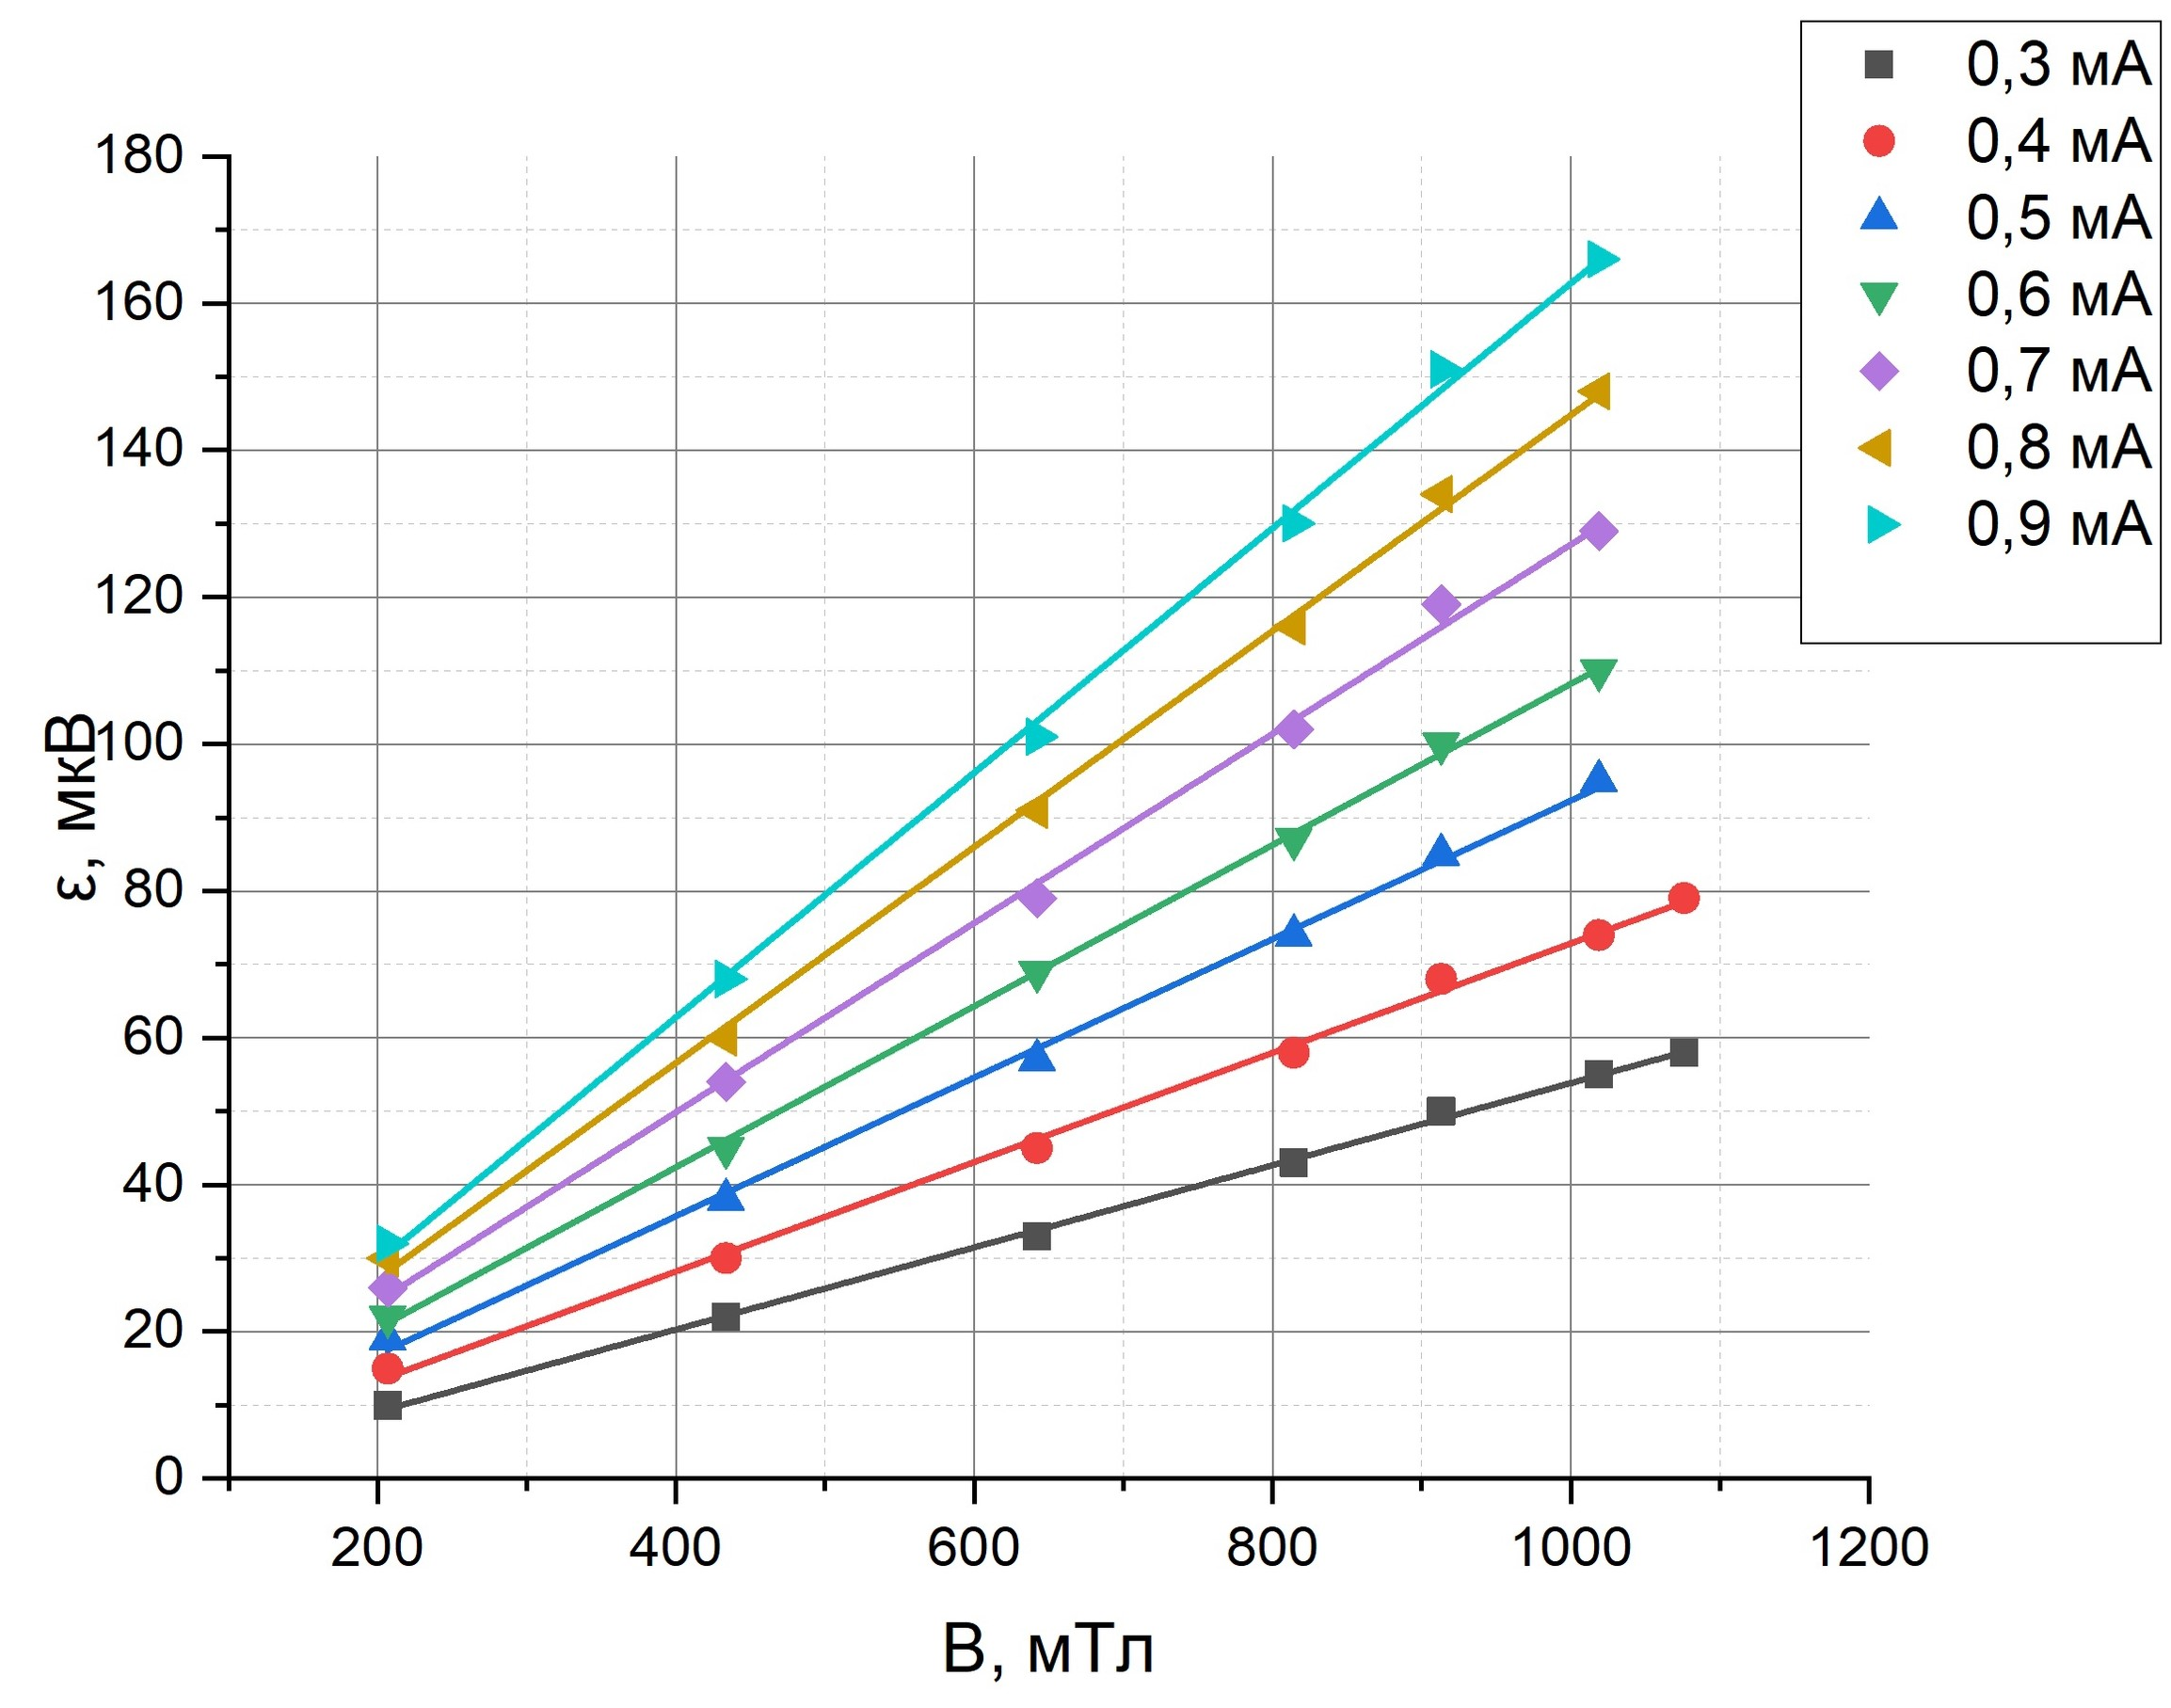
\includegraphics[scale=0.3]{graph2}
		\end{center}
		\caption{Зависимости $\varepsilon(B)$}
		\end{figure}

Из МНК определим угловые коэффициенты наклона прямых -- K -- для каждого тока I. Данные занесем в таблицу.

\newpage

\begin{table}[h]
\caption{}
\begin{center}
\begin{tabular}{|
>{\columncolor[HTML]{92D050}}c |l|l|l|l|l|l|l|}
\hline
\textbf{I, мА}                                                        & 0,3   & 0,4   & 0,5   & 0,6   & 0,7   & 0,8   & 0,9   \\ \hline
\textbf{K, мВ/Тл}                                                     & 0,056 & 0,074 & 0,094 & 0,109 & 0,129 & 0,147 & 0,166 \\ \hline
\multicolumn{1}{|l|}{\cellcolor[HTML]{92D050}\textbf{$\sigma_K$, мВ/Тл}} & 0,001 & 0,002 & 0,002 & 0,001 & 0,003 & 0,003 & 0,003 \\ \hline
\end{tabular}
\end{center}
\end{table}

Построим график K = f(I).
	\begin{figure}[h]
		\begin{center}
		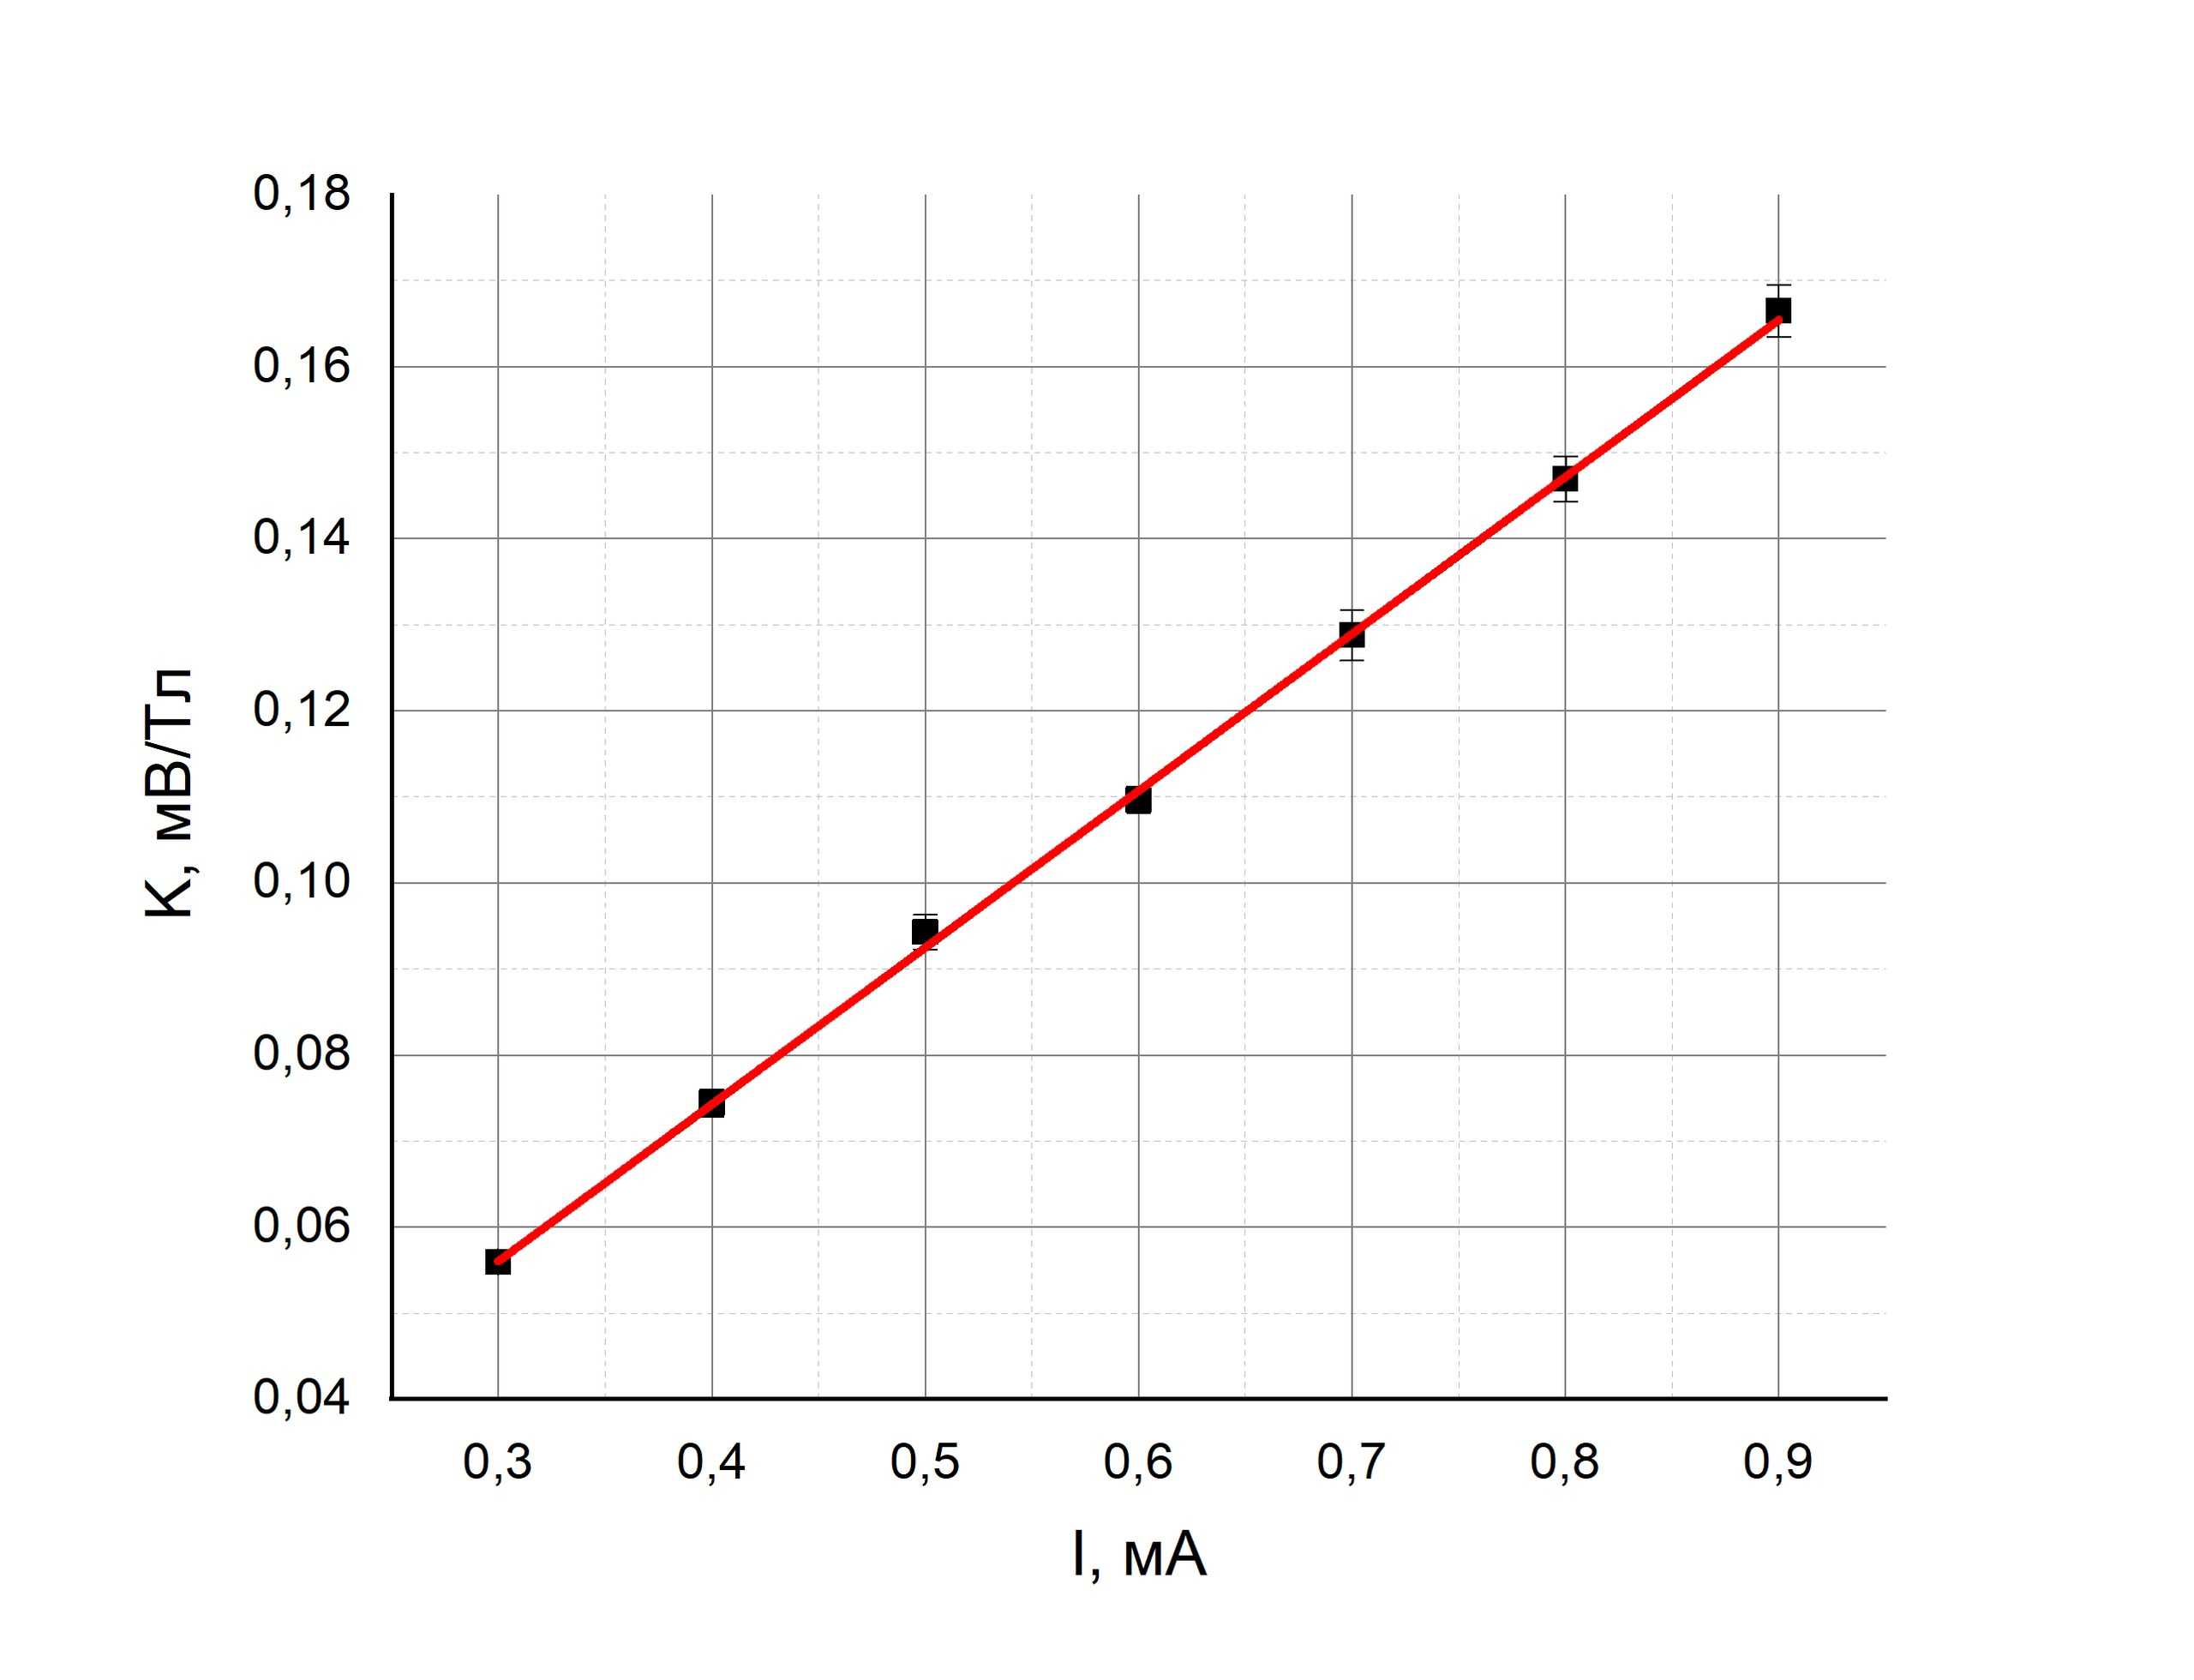
\includegraphics[scale=0.2]{graph3}
		\end{center}
		\caption{Зависимость $K(I)$}
		\end{figure}
		
Из МНК получим наклон прямой:
$$
	\alpha = 0,182 \pm 0,002 \ A * Тл
$$

\newpage

Рассчитаем константу Холла по формуле:
$$
	R_H = \alpha * a \ ,
$$
где а = 2,2 мм -- толщина образца.

\vspace{2 mm}
Погрешность константы Холла определим по формуле:
$$
	\sigma_{R_H} = R_H \frac{\sigma_{\alpha}}{\alpha}
$$

Получим:
$$
	R_H \approx (4,00 \pm 0,04)*10^{-4} \ м^3/Кл
$$

Рассчитаем концентрацию носителей в образце и оценим погрешность по формулам:
$$
	n = \frac{1}{eR_H}
$$
$$	
	\sigma_n = n \frac{\sigma_{R_H}}{R_H}
$$
Получим:
$$
	n \approx (156 \pm 2)*10^{20} \ м^{-3}
$$


\subsection*{Определение удельной проводимости}

При токе через образец I = 1 мА падение напряжения между контактами 3 и 5  $U_{35}$ = 1,729 мВ.По формуле (1) рассчитаем проводимость материала, учитывая что $L_{35}$ = 3 мм, l = 2,5 мм.
$$
	\lambda \approx 315 \ (Ом*м)^{-1}
$$

Оценим погрешность удельной проводимости, учитывая что погрешность вольтметра мала:
$$
	\sigma_{\lambda} = \lambda \frac{\sigma_I}{I} \approx 16 \ (Ом*м)^{-1}
$$

Окончательно получим:
$$
	\lambda = 315 \pm 16 \ (Ом*м)^{-1}
$$

Рассчитаем подвижность b носителей тока и оценим погрешность по формулам

$$
	b = \frac{\sigma}{en} 
$$
$$
	\sigma_b = b * \sqrt{ \frac{\sigma_{\lambda}^2}{\lambda^2} + \frac{\sigma_{n}^2}{n^2}  }
$$
Получим:
$$
	b \approx 0,13 \pm 0,01 \ м^2/(В*с)
$$

\newpage

\subsection*{Определение характера проводимости}
\begin{figure}[h]
		\begin{center}
		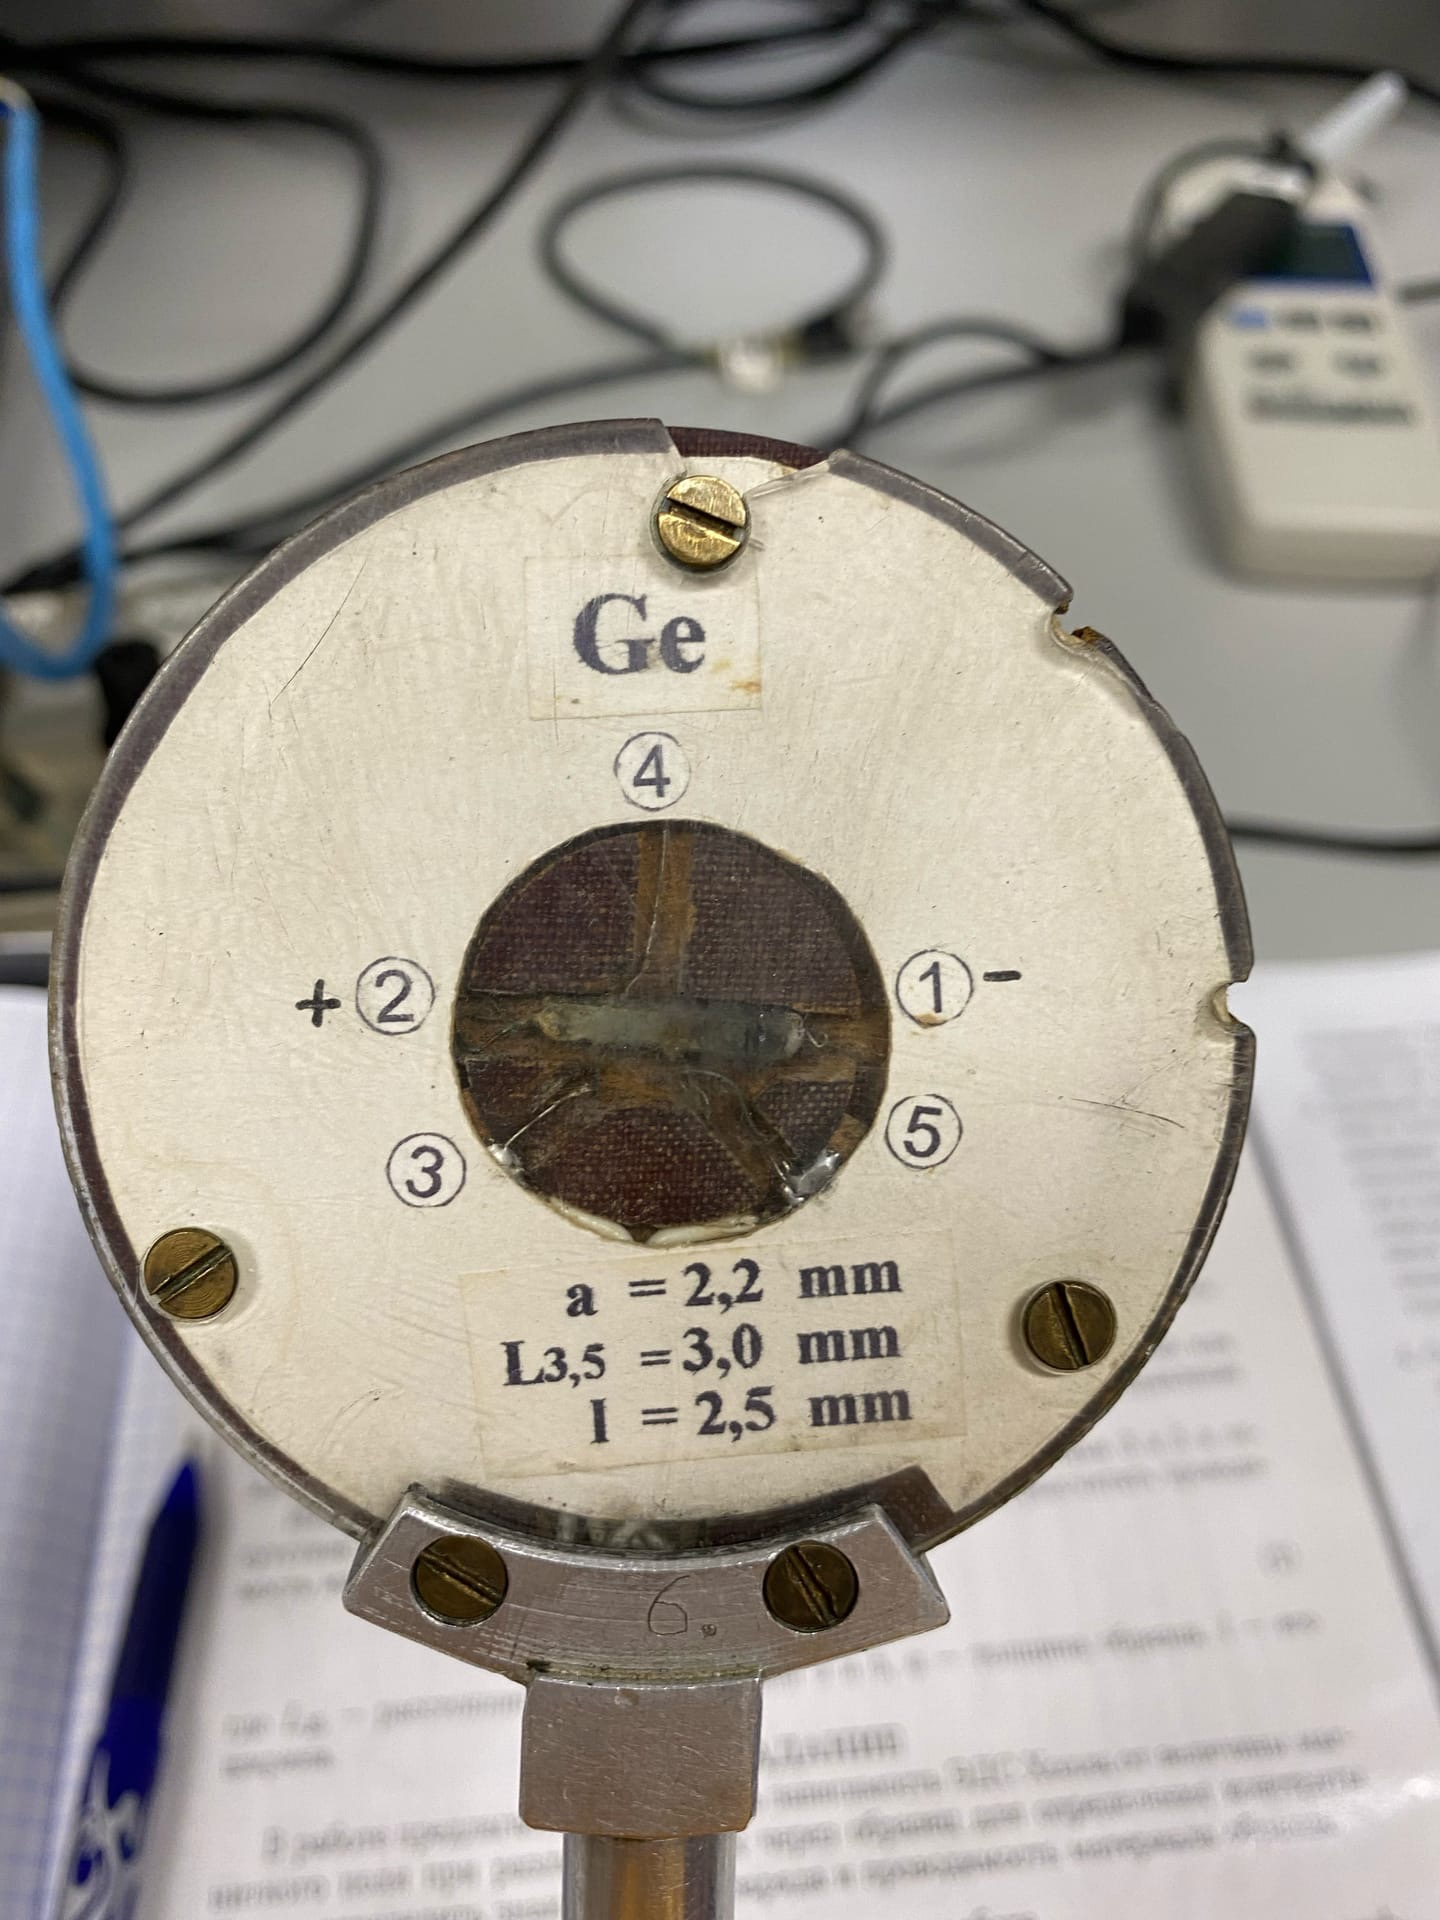
\includegraphics[scale=0.14]{fig2}
		\end{center}
		\caption{Образец легированного Германия}
		\end{figure}
Ток течет от 2 к 1, поле B направлено в плоскость рисунка, из показаний вольтметра -- потенциал 3 -- положителен. По правилу векторного произведения носители заряда "двигаются" к контакту 4, а так как при этом создается положительный потенциал на контакте 3, то можно сделать вывод, что носители заряда - электроны.
\section{Выводы}

\ \ \ 1.В результате работы было получено удельное сопротивление германия, которое по порядку величины совпадает с табличным, но не совпадает численно. Это может быть вызвано тем, что германий содержит примеси (легирован)

2.Также была получена константа Холла для данного образца, которая по порядку величины совпадает с константами Холла для различных легирований Германия.

3.Также был сделан вывод о характере проводимости легированного германия.

\end{document}
